\section{Datenbankmodell}

\subsection{Oracle-SQL-Developer-Data-Modeler}
Der Oracle-SQL-Developer-Data-Modeler ist ein Tool mit einer graphischen Oberfläche und kann kostenlos im Web erworben werden. Es unterstützt die Benutzer einer Oracle-Datenbank beim Erstellen und Bearbeiten der verschiedensten Datenbankmodelle. Der Modeler kann am eigenen Computer laufen, aber auch auf eine Datenbank in einer Cloud zugreifen. (vgl. \cite{modeler})

Das Team verwendete den Oracle-SQL-Developer-Data-Modeler nur, weil es keine anderen Alternativen gab. Es kamen einige Problem, welche viel Zeit in Anspruch nahmen, zum Vorschein, doch es wurden alle gelöst. Das Erstellen der Datenbank war eine große Herausforderung, da die Oberfläche kompliziert gestaltet ist. Außerdem gibt es keine gute Übersichtsansicht der Tabellen. Bei der bestehenden Übersicht sind die Relationen zwischen den Tabellen schwer ablesbar.

Die Übersicht unserer Datenbank haben wir mit der \glqq MySQL-Workbench\grqq{} von der Oracle-Corporation erstellt. Auf dieser Ansicht sind die Relationen schön erkennbar und übersichtlich gestaltet.

\subsection{Tabellen}
Im folgenden Abschnitt werden die Tabellen der Datenbank näher beschrieben. In jeder Tabelle existieren die Felder \glqq created\_at\grqq{} und \glqq updated\_at\grqq{}. Diese werden von Laravel bei der Datenbankerzeugung automatisch generiert und beschreiben, wann der Eintrag erstellt und zuletzt verändert wurde.

\subsubsection{bills}
Die Tabelle dient dazu, die Rechnungen, die von den Lieferanten hochgeladen werden, zu speichern. In dieser wird der Pfad der PDF-Datei sowie das Datum der Rechnung gespeichert. Des Weiteren speichert die Anwendung den Betrag und den Steuerbetrag. Falls der Lieferant der Rechnung eine Benachrichtigung hinzufügt, wird diese ebenfalls zum Rechnungseintrag hinzugefügt. Außerdem wird der Status der Rechnung (gelöscht, geholt, neu) gespeichert. Es existieren Fremdschlüssel-Beziehungen zu der Rechnungsarten-, Währungen-, Firmen- und Lieferanten-Tabelle.
\subsubsection{companies}
In der Firmen-Tabelle werden die Standorte der Firma ELK Fertighaus GmbH gespeichert. Es gibt ein Feld, das die Kürzel der verschiedenen Standorte speichert (001, 002). Dies wird benötigt, um später die XML-Datei bei dem Rechnung holen zu erstellen.
\subsubsection{currencies}
In der Währungen-Tabelle werden die verfügbaren Währungen für die Rechnungen gespeichert. Auch hier existiert ein Feld, das die Abkürzungen der Währungen speichert (EUR, GBP). Dies wird ebenfalls benötigt um die XML-Datei zu generieren.
\subsubsection{billtypes}
In der Rechnungsarten-Tabelle werden die verschiedenen Rechnungstypen (Rechnung, Gutschrift) gespeichert. Das Kürzel-Feld beinhaltet die Abkürzungen der Rechnungsarten (R, G). Diese Tabelle wird ebenfalls zum Erstellen der XML-Datei benötigt.
\subsubsection{users}
In dieser Tabelle werden alle Benutzer der Anwendung gespeichert. Es wird der Benutzername, die E-Mail sowie das Passwort gespeichert. Ebenso wird gespeichert, ob der Benutzer sein Passwort beim Anmelden ändern muss. Zudem werden noch die Berechtigungen der einzelnen Benutzer gesichert (Lieferant, Buchhalter, Administrator). Zudem erhält es ein Feld, das angibt, ob der Benutzer gesperrt ist, daher kann er sich nicht anmelden.
\subsubsection{suppliers}
In der Lieferanten-Tabelle werden die Lieferanten-Informationen gespeichert. Die Informationen der Tabelle werden aus einer Excel-Tabelle, die von der Firma ELK Fertighaus zur Verfügung gestellt wird, gespeist. Es existiert eine Fremdschlüssel-Beziehung zu der Users-Tabelle. Die Tabelle erfüllt den Zweck, dass die Lieferanten-Daten, die einem Benutzer zugehörig sind, auch richtig in der XML-Datei verwendet werden.
\subsubsection{emails}
In dieser Tabelle werden die verwendeten E-Mails und deren Verwendungszweck gespeichert. Es existieren E-Mails zum Versenden und zum Empfangen von Nachrichten.
\newpage 
\subsubsection{password\_criterias}
Diese Tabelle beinhaltet die Passwortkriterien für jede einzelne Benutzergruppe (Administrator, Buchhalter, Lieferant). Es ist festlegbar, ob das Passwort Sonderzeichen, Zahlen, minimale Zeichenanzahl, Groß- und Kleinschreibung enthalten muss. Des Weiteren existiert ein Feld, in welchem Intervall das Passwort geändert werden muss (z.B.: jede Woche).

\subsubsection{jobs}
In dieser Tabelle werden die Jobs gespeichert, die von der Anwendung generiert werden. Zum Beispiel E-Mails. Beim Aktivieren des zugehörigen Artisan-CLI-Befehls werden die Einträge der Tabelle abgearbeitet und anschließend entfernt.
\subsubsection{failed\_jobs}
In dieser Tabelle werden die fehlgeschlagenen Jobs gespeichert, zum Beispiel eine XML-Datei, die versendet werden soll, existiert nicht mehr. Wenn ein Job in der Jobs-Tabelle nicht abgearbeitet werden kann, wird er in diese Tabelle verschoben und zu einem späteren Zeitpunkt abgearbeitet. Damit wird der Geschwindigkeit der Anwendung kein Abbruch getan.

\begin{sidewaysfigure}
\centering
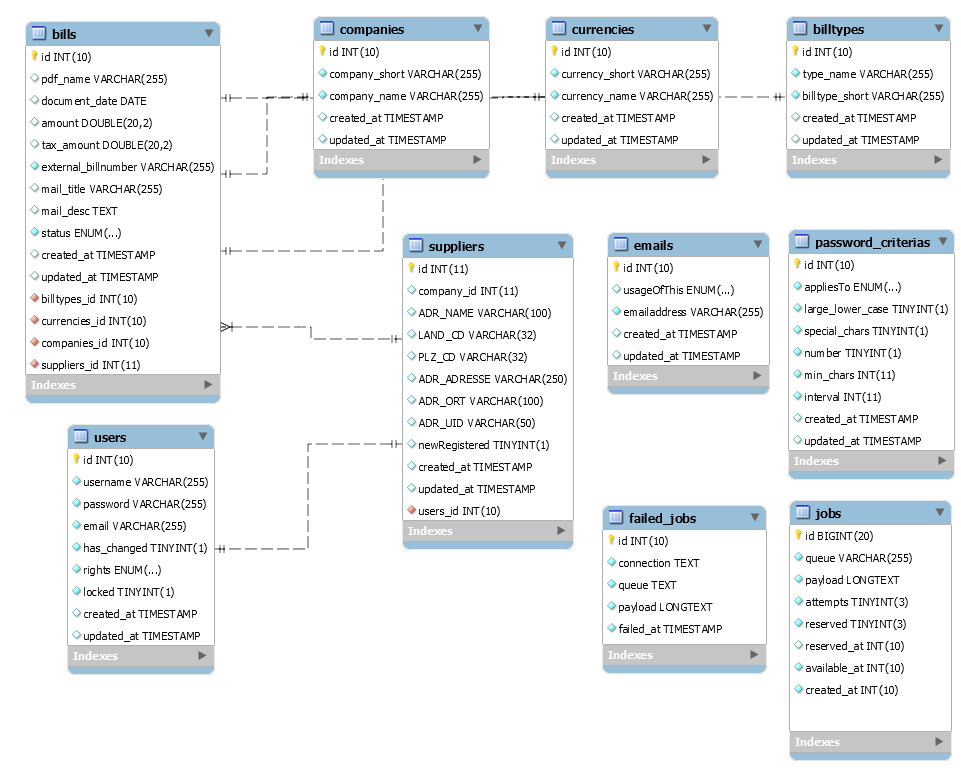
\includegraphics[scale=0.9]{figures/datenbank.PNG}
\caption{ER-Modell der Datenbank}
\label{fig:ermodell} 
\end{sidewaysfigure}